% Created 2018-04-16 Mon 12:46
% Intended LaTeX compiler: pdflatex
\documentclass[10pt]{beamer}
\usepackage[utf8]{inputenc}
\usepackage[T1]{fontenc}
\usepackage{graphicx}
\usepackage{grffile}
\usepackage{longtable}
\usepackage{wrapfig}
\usepackage{rotating}
\usepackage[normalem]{ulem}
\usepackage{amsmath}
\usepackage{textcomp}
\usepackage{amssymb}
\usepackage{capt-of}
\usepackage{hyperref}
\usetheme{Boadilla}
\author{ECON 420: Game Theory}
\date{Spring 2018}
\title{Nash Equilibrium}
\usecolortheme{seagull}
\usefonttheme[onlylarge]{structurebold}
\usefonttheme[onlymath]{serif}
\setbeamerfont*{frametitle}{size=\normalsize,series=\bfseries}
\setbeamertemplate{navigation symbols}{}
\setbeamertemplate{itemize item}[triangle]
\setbeamertemplate{footline}{}
\setbeamertemplate{enumerate items}[default]
\hypersetup{
 pdfauthor={ECON 420: Game Theory},
 pdftitle={Nash Equilibrium},
 pdfkeywords={},
 pdfsubject={},
 pdfcreator={Emacs 25.2.2 (Org mode 9.1.6)}, 
 pdflang={English}}
\begin{document}

\maketitle

\begin{frame}[label={sec:orgf082e89}]{}
\alert{Pick-a-color game}
\begin{itemize}
\item Two types of teams, A and B
\item Your team will play against the other type (A vs B)
\item Each team chooses "white" or "blue"
\item Payoffs for \alert{A} teams:
\begin{itemize}
\item If both teams choose white: 50
\item If both teams choose blue: 25
\item If A chooses white and B chooses blue: 75
\item If A chooses blue and B chooses white: 50
\end{itemize}
\item Payoffs for \alert{B} teams:
\begin{itemize}
\item If both teams choose white: 50
\item If both teams choose blue: 75
\item If A chooses white and B chooses blue: 25
\item If A chooses blue and B chooses white: 50
\end{itemize}
\end{itemize}
\end{frame}

\begin{frame}[label={sec:org5416928}]{}
\alert{Pick-a-color game (version 2)}
\begin{itemize}
\item Each team chooses "orange" or "black"
\item Payoffs for \alert{A} teams:
\begin{itemize}
\item If both teams choose orange: 75
\item If both teams choose black: 50
\item If A chooses orange and B chooses black: 25
\item If A chooses black and B chooses orange: 50
\end{itemize}
\item Payoffs for \alert{B} teams:
\begin{itemize}
\item If both teams choose orange: 25
\item If both teams choose black: 50
\item If A chooses orange and B chooses black: 75
\item If A chooses black and B chooses orange: 50
\end{itemize}
\end{itemize}
\end{frame}

\begin{frame}[label={sec:org523579e}]{Pick a color, normal form}
\end{frame}

\begin{frame}[label={sec:orgd86dc42}]{Version 2, normal form}
\end{frame}

\begin{frame}[label={sec:orgbd1f451}]{}
\alert{Prisoners' Dilemma}
\begin{itemize}
\item The story:
\begin{itemize}
\item Husband and wife are arrested for a crime and interrogated separately
\item Both must choose to confess to the crime or deny that they committed the crime
\item If both deny, serve 3 years for a crime that police can prove
\item A confession is "rewarded" by police if it helps convict the other partner (who denies)
\item If both confess, both serve a long sentence
\end{itemize}
\end{itemize}
\end{frame}

\begin{frame}[label={sec:orgc929148}]{Prisoners' dilemma}
\begin{center}
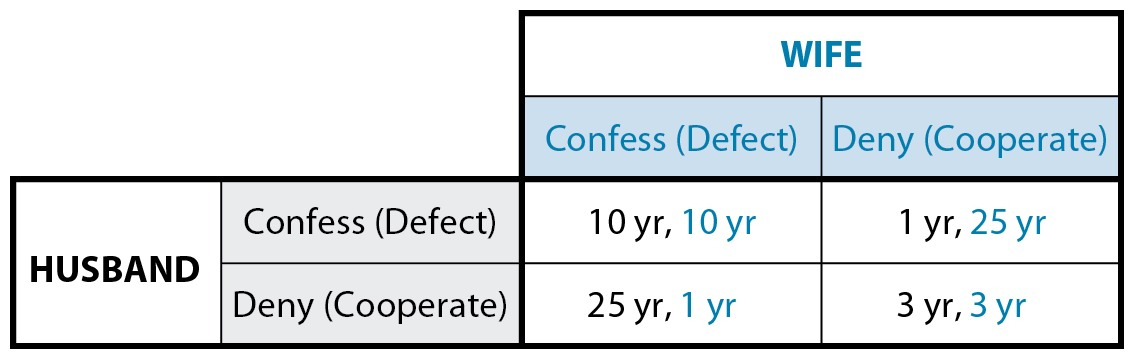
\includegraphics[width=.75\textwidth]{./img/GAMES4_FIG04.04.jpg}
\end{center}
\end{frame}

\begin{frame}[label={sec:org63400c8}]{}
\alert{Best responses}
\begin{enumerate}
\item Suppose husband believes wife will confess. What is his best response?
\item Suppose husband believes wife will deny. What is his best response?
\end{enumerate}
\end{frame}

\begin{frame}[label={sec:org7b31583}]{}
\alert{Dominance}
\begin{itemize}
\item If a strategy is \emph{always} a best response, that strategy is a \emph{dominant} strategy
\item If a strategy is \emph{never} a best response, that strategy is a \emph{dominated} strategy
\item If both players have a dominant strategy, then these strategies define the Nash equilibrium
\item In the prisoners' dilemma, confess is a dominant strategy (deny is dominated)
\item What about pick a color?
\end{itemize}
\end{frame}

\begin{frame}[label={sec:orge55f229}]{}
\alert{Prisoners' dilemma}
\begin{itemize}
\item Both players have a dominant strategy
\item Dominance solution is worse for both players than outcome where both cooperate with each other
\item The outcome that obtains from rational play (and in practice!) is a bad outcome for the players
\end{itemize}
\end{frame}

\begin{frame}[label={sec:orgdfbe306}]{Fiscal and monetary policy game}
\begin{center}
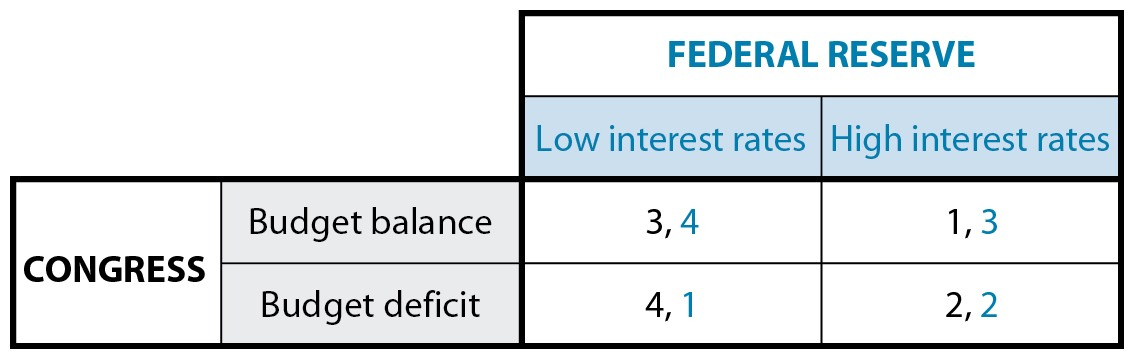
\includegraphics[width=.75\textwidth]{./img/GAMES4_FIG04.05.jpg}
\end{center}
\end{frame}

\begin{frame}[label={sec:org32eef70}]{}
\alert{One player has a dominant strategy}
\begin{itemize}
\item Congress has a dominant strategy, Fed does not
\item But Fed knows that Congress has dominant strategy
\item Fed can choose the best response to Congress's dominant strategy
\end{itemize}
\end{frame}

\begin{frame}[label={sec:orgd7940a1}]{}
\alert{Successive elimination of dominated strategies}
\begin{itemize}
\item If a strategy is dominated, then it won't be played at the equilibrium
\begin{itemize}
\item Rational players won't play dominated strategies, other rational players know this about each other
\end{itemize}
\item Removing dominated strategies can simplify the game, makes finding Nash equilibrium easier
\item A game is \emph{dominance solvable} if successive elimination of dominated strategies ends in a unique outcome (the Nash equilibrium)
\end{itemize}
\end{frame}


\begin{frame}[label={sec:orgfdf85bf}]{}
\begin{center}
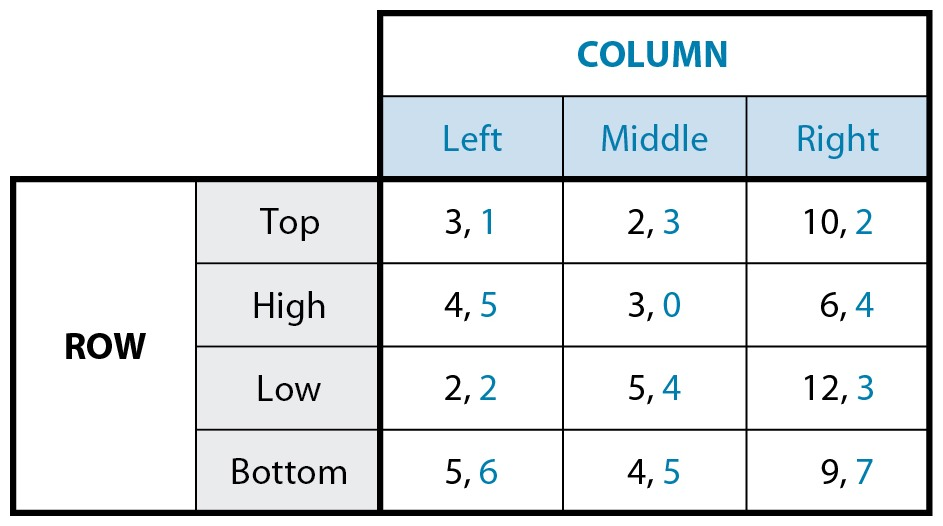
\includegraphics[width=.75\textwidth]{./img/GAMES4_FIG04.01.jpg}
\end{center}
\end{frame}


\begin{frame}[label={sec:orgaf8fc16}]{}
\alert{Weak dominance}
\begin{itemize}
\item A strategy is \emph{weakly dominant} if it never yields a worse outcome than any other strategy
\begin{itemize}
\item Allows for "ties" in payoffs
\end{itemize}
\item Can eliminate weekly dominated strategies to find equilibrium as well
\end{itemize}
\end{frame}

\begin{frame}[label={sec:orgdecf9cf}]{}
\begin{center}
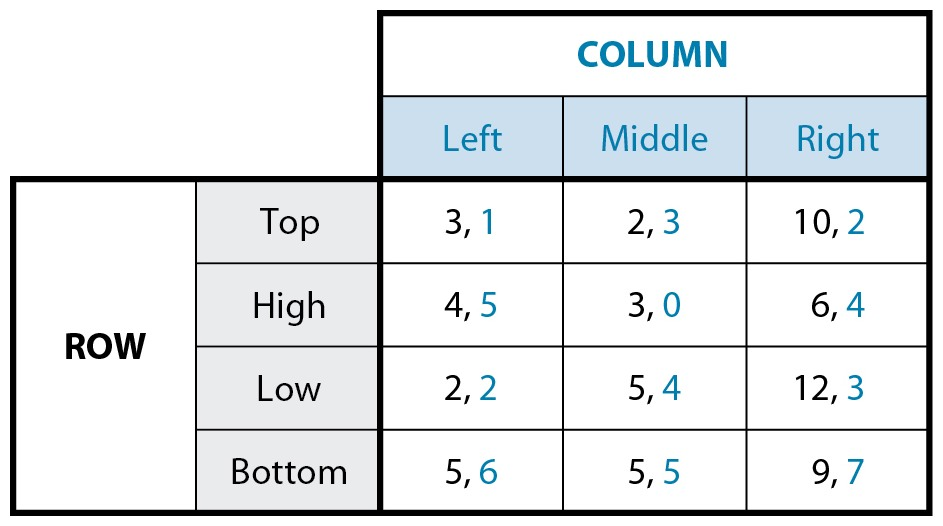
\includegraphics[width=.75\textwidth]{./img/GAMES4_FIG04.03.jpg}
\end{center}
\end{frame}



\begin{frame}[label={sec:org8cdde7c}]{}
\alert{Elimination of weakly dominated strategies}
\begin{itemize}
\item We can sometimes find a Nash equilibrium by eliminating weakly dominated strategies
\item However, we can also eliminate other Nash equilibrium with this strategy!
\end{itemize}
\end{frame}

\begin{frame}[label={sec:org18cf05c}]{}
\begin{center}
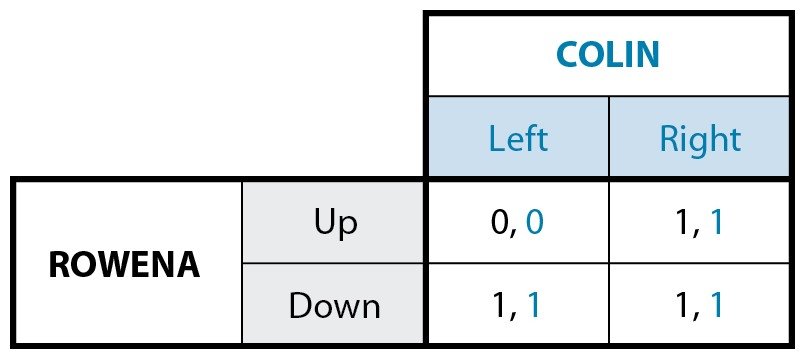
\includegraphics[width=.75\textwidth]{./img/GAMES4_FIG04.06.jpg}
\end{center}
\end{frame}

\begin{frame}[label={sec:org15e27e9}]{}
\alert{Best response analysis}
\begin{itemize}
\item The Nash equilibrium is a mutual best response
\item We can find the best response for each player for any given opponent strategy
\item We can use this to find a Nash equilibrium:
\begin{itemize}
\item Find the best responses for each player for \emph{all possible} opponent strategies
\item If one outcome is a best response for both players, then it must be a Nash equilibrium
\end{itemize}
\end{itemize}
\end{frame}

\begin{frame}[label={sec:org54e7d29}]{}
\begin{center}
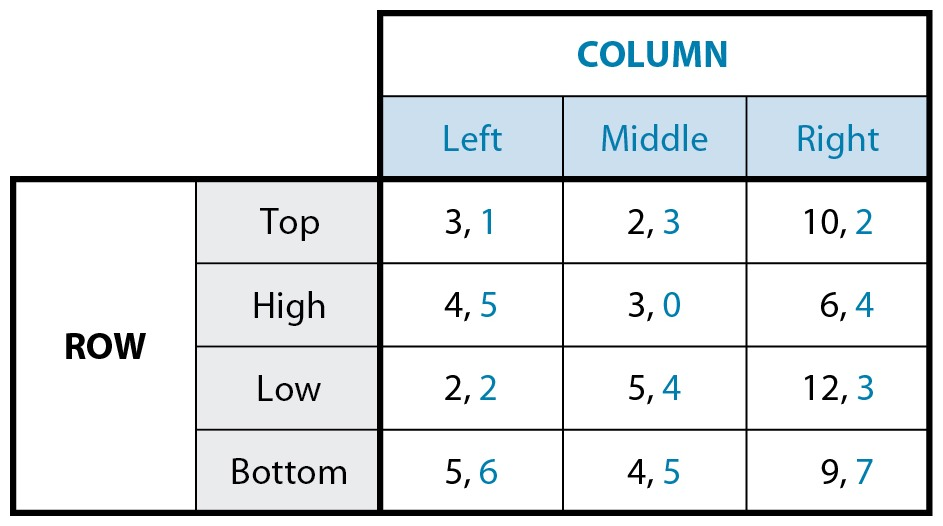
\includegraphics[width=.75\textwidth]{./img/GAMES4_FIG04.01.jpg}
\end{center}
\end{frame}

\begin{frame}[label={sec:org6733a4b}]{}
\begin{center}
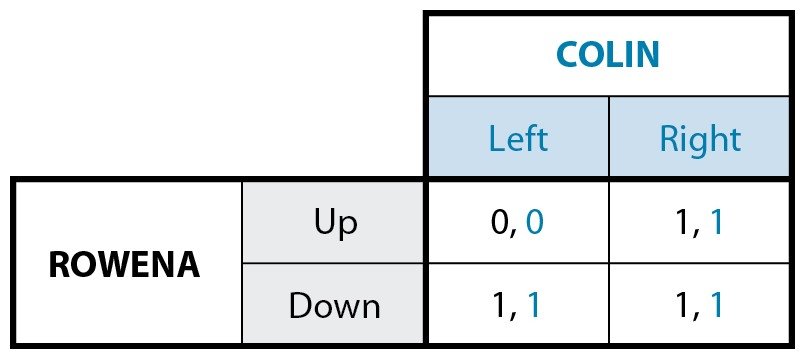
\includegraphics[width=.75\textwidth]{./img/GAMES4_FIG04.06.jpg}
\end{center}
\end{frame}


\begin{frame}[label={sec:orgc72f2ae}]{}
\alert{Three player games}
\begin{itemize}
\item We need three dimensions to describe the payoff space with three players
\item Alternatively, write multiple game matrices for two players, given the choices of a third player
\item Use best response analysis as before: find best response given strategies of \emph{both} of the other players
\end{itemize}
\end{frame}

\begin{frame}[label={sec:org60c7691}]{}
\begin{center}
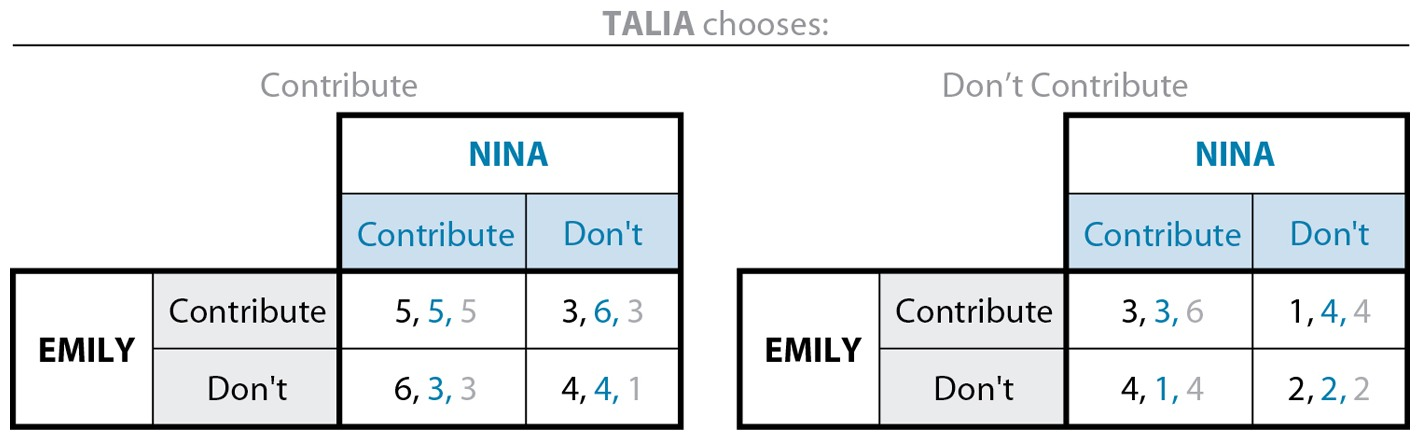
\includegraphics[width=.75\textwidth]{./img/GAMES4_FIG04.08.jpg}
\end{center}
\end{frame}

\begin{frame}[label={sec:orgc8f0320}]{}
\alert{Pure coordination} 
\begin{itemize}
\item Many games have multiple Nash equilibria
\item If the payoffs are identical across equilibria, then it is a game of \emph{pure coordination}
\end{itemize}
\end{frame}

\begin{frame}[label={sec:org1252543}]{}
\alert{Pure coordination example}
\begin{itemize}
\item You are to meet someone in Corvallis. You have not been instructed where to
\end{itemize}
meet, you have no prior understanding with the person on where to meet, and
you cannot communicate with each other. You are simply told that you will
have to guess where to meet, that the other person is being told the same
thing, and that you will just have to try to make your guesses coincide. Where
do you go?
\end{frame}

\begin{frame}[label={sec:orgb33307b}]{Games with no pure strategy equilibrium}
\begin{center}
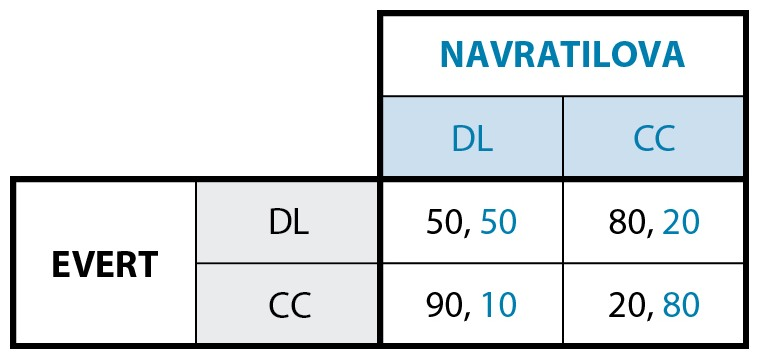
\includegraphics[width=.75\textwidth]{./img/GAMES4_FIG04.14.jpg}
\end{center}
\end{frame}

\begin{frame}[label={sec:org95a96c1}]{}
\alert{Games with no pure strategy equilibrium}
\begin{itemize}
\item What should players do?
\item More importantly: What \emph{shouldn't} players do?
\end{itemize}
\end{frame}
\end{document}